\documentclass[conference]{IEEEtran}
\IEEEoverridecommandlockouts
% Shared by bpp_v3_conf.tex and bpp_v3_journal.tex
\usepackage{amsmath,amssymb}
\usepackage{graphicx}
\usepackage{booktabs}
\usepackage{xurl}
\usepackage{cite}
\usepackage{xspace}
\usepackage[table]{xcolor}
\graphicspath{{figures/}}

% System name in one place: change here to rename everywhere.
\newcommand{\sysname}{BioPathNet++\xspace}

% Every number below is generated by `python -m bpp.analyze` from the run logs;
% never type a result by hand in the papers.
\newcommand{\MainValidMrr}{0.394}
\newcommand{\MainValidMrrSd}{0.003}
\newcommand{\MainValidHitsOne}{0.353}
\newcommand{\MainValidHitsOneSd}{0.008}
\newcommand{\MainValidHitsTen}{0.456}
\newcommand{\MainValidHitsTenSd}{0.018}
\newcommand{\MainValidHitsHundred}{0.669}
\newcommand{\MainValidHitsHundredSd}{0.021}
\newcommand{\MainValidAuroc}{0.938}
\newcommand{\MainValidAurocSd}{0.001}
\newcommand{\MainValidAuprc}{0.424}
\newcommand{\MainValidAuprcSd}{0.005}
\newcommand{\MainValidAurocHard}{0.799}
\newcommand{\MainValidAurocHardSd}{0.010}
\newcommand{\MainValidAurocDeg}{0.886}
\newcommand{\MainValidAurocDegSd}{0.010}
\newcommand{\MainValidAnyTen}{56}
\newcommand{\MainTargetsMrr}{0.475}
\newcommand{\MainTargetsMrrSd}{0.017}
\newcommand{\MainTargetsHitsOne}{0.396}
\newcommand{\MainTargetsHitsOneSd}{0.038}
\newcommand{\MainTargetsHitsTen}{0.648}
\newcommand{\MainTargetsHitsTenSd}{0.033}
\newcommand{\MainTargetsHitsHundred}{0.716}
\newcommand{\MainTargetsHitsHundredSd}{0.016}
\newcommand{\MainTargetsAuroc}{0.982}
\newcommand{\MainTargetsAurocSd}{0.008}
\newcommand{\MainTargetsAuprc}{0.594}
\newcommand{\MainTargetsAuprcSd}{0.010}
\newcommand{\MainTargetsAurocHard}{0.892}
\newcommand{\MainTargetsAurocHardSd}{0.020}
\newcommand{\MainTargetsAurocDeg}{0.954}
\newcommand{\MainTargetsAurocDegSd}{0.031}
\newcommand{\MainTargetsAnyTen}{83}
\newcommand{\MainSeeds}{3}
\newcommand{\PathsValidMrr}{0.405}
\newcommand{\PathsValidMrrSd}{0.013}
\newcommand{\PathsValidHitsOne}{0.363}
\newcommand{\PathsValidHitsOneSd}{0.019}
\newcommand{\PathsValidHitsTen}{0.479}
\newcommand{\PathsValidHitsTenSd}{0.025}
\newcommand{\PathsValidHitsHundred}{0.663}
\newcommand{\PathsValidHitsHundredSd}{0.018}
\newcommand{\PathsValidAuroc}{0.946}
\newcommand{\PathsValidAurocSd}{0.004}
\newcommand{\PathsValidAuprc}{0.443}
\newcommand{\PathsValidAuprcSd}{0.010}
\newcommand{\PathsValidAurocHard}{0.829}
\newcommand{\PathsValidAurocHardSd}{0.011}
\newcommand{\PathsValidAurocDeg}{0.888}
\newcommand{\PathsValidAurocDegSd}{0.009}
\newcommand{\PathsValidAnyTen}{59}
\newcommand{\PathsTargetsMrr}{0.463}
\newcommand{\PathsTargetsMrrSd}{0.087}
\newcommand{\PathsTargetsHitsOne}{0.375}
\newcommand{\PathsTargetsHitsOneSd}{0.134}
\newcommand{\PathsTargetsHitsTen}{0.657}
\newcommand{\PathsTargetsHitsTenSd}{0.025}
\newcommand{\PathsTargetsHitsHundred}{0.738}
\newcommand{\PathsTargetsHitsHundredSd}{0.023}
\newcommand{\PathsTargetsAuroc}{0.986}
\newcommand{\PathsTargetsAurocSd}{0.004}
\newcommand{\PathsTargetsAuprc}{0.577}
\newcommand{\PathsTargetsAuprcSd}{0.054}
\newcommand{\PathsTargetsAurocHard}{0.907}
\newcommand{\PathsTargetsAurocHardSd}{0.007}
\newcommand{\PathsTargetsAurocDeg}{0.968}
\newcommand{\PathsTargetsAurocDegSd}{0.015}
\newcommand{\PathsTargetsAnyTen}{83}
\newcommand{\PathsSeeds}{3}
\newcommand{\PriorValidMrr}{0.303}
\newcommand{\PriorValidMrrSd}{--}
\newcommand{\PriorValidHitsOne}{0.265}
\newcommand{\PriorValidHitsOneSd}{--}
\newcommand{\PriorValidHitsTen}{0.353}
\newcommand{\PriorValidHitsTenSd}{--}
\newcommand{\PriorValidHitsHundred}{0.536}
\newcommand{\PriorValidHitsHundredSd}{--}
\newcommand{\PriorValidAuroc}{0.884}
\newcommand{\PriorValidAurocSd}{--}
\newcommand{\PriorValidAuprc}{0.334}
\newcommand{\PriorValidAuprcSd}{--}
\newcommand{\PriorValidAurocHard}{0.707}
\newcommand{\PriorValidAurocHardSd}{--}
\newcommand{\PriorValidAurocDeg}{0.843}
\newcommand{\PriorValidAurocDegSd}{--}
\newcommand{\PriorValidAnyTen}{46}
\newcommand{\PriorTargetsMrr}{0.322}
\newcommand{\PriorTargetsMrrSd}{--}
\newcommand{\PriorTargetsHitsOne}{0.243}
\newcommand{\PriorTargetsHitsOneSd}{--}
\newcommand{\PriorTargetsHitsTen}{0.483}
\newcommand{\PriorTargetsHitsTenSd}{--}
\newcommand{\PriorTargetsHitsHundred}{0.718}
\newcommand{\PriorTargetsHitsHundredSd}{--}
\newcommand{\PriorTargetsAuroc}{0.955}
\newcommand{\PriorTargetsAurocSd}{--}
\newcommand{\PriorTargetsAuprc}{0.443}
\newcommand{\PriorTargetsAuprcSd}{--}
\newcommand{\PriorTargetsAurocHard}{0.782}
\newcommand{\PriorTargetsAurocHardSd}{--}
\newcommand{\PriorTargetsAurocDeg}{0.909}
\newcommand{\PriorTargetsAurocDegSd}{--}
\newcommand{\PriorTargetsAnyTen}{83}
\newcommand{\PriorSeeds}{1}
\newcommand{\NoautoValidMrr}{0.454}
\newcommand{\NoautoValidMrrSd}{--}
\newcommand{\NoautoValidHitsOne}{0.400}
\newcommand{\NoautoValidHitsOneSd}{--}
\newcommand{\NoautoValidHitsTen}{0.557}
\newcommand{\NoautoValidHitsTenSd}{--}
\newcommand{\NoautoValidHitsHundred}{0.719}
\newcommand{\NoautoValidHitsHundredSd}{--}
\newcommand{\NoautoValidAuroc}{0.946}
\newcommand{\NoautoValidAurocSd}{--}
\newcommand{\NoautoValidAuprc}{0.489}
\newcommand{\NoautoValidAuprcSd}{--}
\newcommand{\NoautoValidAurocHard}{0.838}
\newcommand{\NoautoValidAurocHardSd}{--}
\newcommand{\NoautoValidAurocDeg}{0.891}
\newcommand{\NoautoValidAurocDegSd}{--}
\newcommand{\NoautoValidAnyTen}{70}
\newcommand{\NoautoTargetsMrr}{0.473}
\newcommand{\NoautoTargetsMrrSd}{--}
\newcommand{\NoautoTargetsHitsOne}{0.404}
\newcommand{\NoautoTargetsHitsOneSd}{--}
\newcommand{\NoautoTargetsHitsTen}{0.628}
\newcommand{\NoautoTargetsHitsTenSd}{--}
\newcommand{\NoautoTargetsHitsHundred}{0.711}
\newcommand{\NoautoTargetsHitsHundredSd}{--}
\newcommand{\NoautoTargetsAuroc}{0.975}
\newcommand{\NoautoTargetsAurocSd}{--}
\newcommand{\NoautoTargetsAuprc}{0.576}
\newcommand{\NoautoTargetsAuprcSd}{--}
\newcommand{\NoautoTargetsAurocHard}{0.899}
\newcommand{\NoautoTargetsAurocHardSd}{--}
\newcommand{\NoautoTargetsAurocDeg}{0.914}
\newcommand{\NoautoTargetsAurocDegSd}{--}
\newcommand{\NoautoTargetsAnyTen}{83}
\newcommand{\NoautoAreaMrr}{0.485}
\newcommand{\NoautoAreaMrrSd}{--}
\newcommand{\NoautoAreaHitsOne}{0.406}
\newcommand{\NoautoAreaHitsOneSd}{--}
\newcommand{\NoautoAreaHitsTen}{0.608}
\newcommand{\NoautoAreaHitsTenSd}{--}
\newcommand{\NoautoAreaHitsHundred}{0.717}
\newcommand{\NoautoAreaHitsHundredSd}{--}
\newcommand{\NoautoAreaAuroc}{0.947}
\newcommand{\NoautoAreaAurocSd}{--}
\newcommand{\NoautoAreaAuprc}{0.528}
\newcommand{\NoautoAreaAuprcSd}{--}
\newcommand{\NoautoAreaAurocHard}{0.816}
\newcommand{\NoautoAreaAurocHardSd}{--}
\newcommand{\NoautoAreaAurocDeg}{0.913}
\newcommand{\NoautoAreaAurocDegSd}{--}
\newcommand{\NoautoAreaAnyTen}{76}
\newcommand{\NoautoSeeds}{1}
\newcommand{\KnnValidMrr}{0.281}
\newcommand{\KnnValidHitsTen}{0.350}
\newcommand{\KnnValidAuroc}{0.860}
\newcommand{\KnnValidAurocHard}{0.661}
\newcommand{\KnnValidAnyTen}{44}
\newcommand{\KnnTargetsMrr}{0.296}
\newcommand{\KnnTargetsHitsTen}{0.424}
\newcommand{\KnnTargetsAuroc}{0.962}
\newcommand{\KnnTargetsAurocHard}{0.778}
\newcommand{\KnnTargetsAnyTen}{67}
\newcommand{\PopValidMrr}{0.046}
\newcommand{\PopValidHitsTen}{0.049}
\newcommand{\PopValidAuroc}{0.830}
\newcommand{\PopValidAurocHard}{0.476}
\newcommand{\PopValidAnyTen}{15}
\newcommand{\PopTargetsMrr}{0.099}
\newcommand{\PopTargetsHitsTen}{0.148}
\newcommand{\PopTargetsAuroc}{0.905}
\newcommand{\PopTargetsAurocHard}{0.460}
\newcommand{\PopTargetsAnyTen}{50}
\newcommand{\RandValidMrr}{0.001}
\newcommand{\RandValidHitsTen}{0.002}
\newcommand{\RandValidAuroc}{0.471}
\newcommand{\RandValidAurocHard}{0.488}
\newcommand{\RandValidAnyTen}{1}
\newcommand{\RandTargetsMrr}{0.001}
\newcommand{\RandTargetsHitsTen}{0.000}
\newcommand{\RandTargetsAuroc}{0.476}
\newcommand{\RandTargetsAurocHard}{0.488}
\newcommand{\RandTargetsAnyTen}{0}
\newcommand{\DegValidMrr}{0.004}
\newcommand{\DegValidHitsTen}{0.003}
\newcommand{\DegValidAuroc}{0.783}
\newcommand{\DegValidAurocHard}{0.421}
\newcommand{\DegValidAnyTen}{1}
\newcommand{\DegTargetsMrr}{0.003}
\newcommand{\DegTargetsHitsTen}{0.000}
\newcommand{\DegTargetsAuroc}{0.732}
\newcommand{\DegTargetsAurocHard}{0.404}
\newcommand{\DegTargetsAnyTen}{0}
\newcommand{\NoautoKnnValidMrr}{0.347}
\newcommand{\NoautoKnnValidHitsTen}{0.407}
\newcommand{\NoautoKnnValidAuroc}{0.890}
\newcommand{\NoautoKnnValidAurocHard}{0.748}
\newcommand{\NoautoKnnValidAnyTen}{53}
\newcommand{\NoautoKnnTargetsMrr}{0.273}
\newcommand{\NoautoKnnTargetsHitsTen}{0.594}
\newcommand{\NoautoKnnTargetsAuroc}{0.857}
\newcommand{\NoautoKnnTargetsAurocHard}{0.790}
\newcommand{\NoautoKnnTargetsAnyTen}{83}
\newcommand{\NoautoKnnAreaMrr}{0.311}
\newcommand{\NoautoKnnAreaHitsTen}{0.469}
\newcommand{\NoautoKnnAreaAuroc}{0.832}
\newcommand{\NoautoKnnAreaAurocHard}{0.712}
\newcommand{\NoautoKnnAreaAnyTen}{57}
\newcommand{\NoautoPopValidMrr}{0.054}
\newcommand{\NoautoPopValidHitsTen}{0.054}
\newcommand{\NoautoPopValidAuroc}{0.871}
\newcommand{\NoautoPopValidAurocHard}{0.639}
\newcommand{\NoautoPopValidAnyTen}{12}
\newcommand{\NoautoPopTargetsMrr}{0.093}
\newcommand{\NoautoPopTargetsHitsTen}{0.148}
\newcommand{\NoautoPopTargetsAuroc}{0.799}
\newcommand{\NoautoPopTargetsAurocHard}{0.519}
\newcommand{\NoautoPopTargetsAnyTen}{50}
\newcommand{\NoautoPopAreaMrr}{0.260}
\newcommand{\NoautoPopAreaHitsTen}{0.346}
\newcommand{\NoautoPopAreaAuroc}{0.808}
\newcommand{\NoautoPopAreaAurocHard}{0.604}
\newcommand{\NoautoPopAreaAnyTen}{48}
\newcommand{\NoautoRandValidMrr}{0.001}
\newcommand{\NoautoRandValidHitsTen}{0.005}
\newcommand{\NoautoRandValidAuroc}{0.428}
\newcommand{\NoautoRandValidAurocHard}{0.443}
\newcommand{\NoautoRandValidAnyTen}{2}
\newcommand{\NoautoRandTargetsMrr}{0.001}
\newcommand{\NoautoRandTargetsHitsTen}{0.000}
\newcommand{\NoautoRandTargetsAuroc}{0.476}
\newcommand{\NoautoRandTargetsAurocHard}{0.488}
\newcommand{\NoautoRandTargetsAnyTen}{0}
\newcommand{\NoautoRandAreaMrr}{0.000}
\newcommand{\NoautoRandAreaHitsTen}{0.000}
\newcommand{\NoautoRandAreaAuroc}{0.419}
\newcommand{\NoautoRandAreaAurocHard}{0.436}
\newcommand{\NoautoRandAreaAnyTen}{0}
\newcommand{\NoautoDegValidMrr}{0.003}
\newcommand{\NoautoDegValidHitsTen}{0.001}
\newcommand{\NoautoDegValidAuroc}{0.778}
\newcommand{\NoautoDegValidAurocHard}{0.435}
\newcommand{\NoautoDegValidAnyTen}{2}
\newcommand{\NoautoDegTargetsMrr}{0.003}
\newcommand{\NoautoDegTargetsHitsTen}{0.000}
\newcommand{\NoautoDegTargetsAuroc}{0.732}
\newcommand{\NoautoDegTargetsAurocHard}{0.404}
\newcommand{\NoautoDegTargetsAnyTen}{0}
\newcommand{\NoautoDegAreaMrr}{0.003}
\newcommand{\NoautoDegAreaHitsTen}{0.000}
\newcommand{\NoautoDegAreaAuroc}{0.820}
\newcommand{\NoautoDegAreaAurocHard}{0.443}
\newcommand{\NoautoDegAreaAnyTen}{0}
\newcommand{\DiffMainKnnValid}{+0.113}
\newcommand{\PbootMainKnnValid}{$<$0.001}
\newcommand{\PwilMainKnnValid}{$<$0.001}
\newcommand{\DiffLoMainKnnValid}{+0.056}
\newcommand{\DiffHiMainKnnValid}{+0.179}
\newcommand{\WinsMainKnnValid}{43}
\newcommand{\TiesMainKnnValid}{13}
\newcommand{\LossesMainKnnValid}{12}
\newcommand{\DiffMainKnnTargets}{+0.179}
\newcommand{\PbootMainKnnTargets}{$=$0.043}
\newcommand{\PwilMainKnnTargets}{$=$0.188}
\newcommand{\DiffLoMainKnnTargets}{-0.027}
\newcommand{\DiffHiMainKnnTargets}{+0.370}
\newcommand{\WinsMainKnnTargets}{4}
\newcommand{\TiesMainKnnTargets}{1}
\newcommand{\LossesMainKnnTargets}{1}
\newcommand{\DiffMainPathsValid}{-0.010}
\newcommand{\PbootMainPathsValid}{$=$0.752}
\newcommand{\PwilMainPathsValid}{$=$0.148}
\newcommand{\DiffLoMainPathsValid}{-0.043}
\newcommand{\DiffHiMainPathsValid}{+0.021}
\newcommand{\WinsMainPathsValid}{19}
\newcommand{\TiesMainPathsValid}{14}
\newcommand{\LossesMainPathsValid}{35}
\newcommand{\DiffMainPathsTargets}{+0.011}
\newcommand{\PbootMainPathsTargets}{$=$0.359}
\newcommand{\PwilMainPathsTargets}{$=$0.625}
\newcommand{\DiffLoMainPathsTargets}{-0.105}
\newcommand{\DiffHiMainPathsTargets}{+0.129}
\newcommand{\WinsMainPathsTargets}{3}
\newcommand{\TiesMainPathsTargets}{1}
\newcommand{\LossesMainPathsTargets}{2}
\newcommand{\DiffMainNoautoTargets}{+0.002}
\newcommand{\PbootMainNoautoTargets}{$=$0.435}
\newcommand{\PwilMainNoautoTargets}{$=$0.625}
\newcommand{\DiffLoMainNoautoTargets}{-0.090}
\newcommand{\DiffHiMainNoautoTargets}{+0.078}
\newcommand{\WinsMainNoautoTargets}{4}
\newcommand{\TiesMainNoautoTargets}{1}
\newcommand{\LossesMainNoautoTargets}{1}
\newcommand{\DiffNoautoKnnArea}{+0.174}
\newcommand{\PbootNoautoKnnArea}{$=$0.005}
\newcommand{\PwilNoautoKnnArea}{$=$0.085}
\newcommand{\DiffLoNoautoKnnArea}{+0.033}
\newcommand{\DiffHiNoautoKnnArea}{+0.326}
\newcommand{\WinsNoautoKnnArea}{12}
\newcommand{\TiesNoautoKnnArea}{3}
\newcommand{\LossesNoautoKnnArea}{6}
\newcommand{\DiffPathsKnnValid}{+0.124}
\newcommand{\PbootPathsKnnValid}{$<$0.001}
\newcommand{\PwilPathsKnnValid}{$<$0.001}
\newcommand{\DiffLoPathsKnnValid}{+0.057}
\newcommand{\DiffHiPathsKnnValid}{+0.197}
\newcommand{\WinsPathsKnnValid}{44}
\newcommand{\TiesPathsKnnValid}{13}
\newcommand{\LossesPathsKnnValid}{11}
\newcommand{\DiffMainPriorValid}{+0.092}
\newcommand{\PbootMainPriorValid}{$<$0.001}
\newcommand{\PwilMainPriorValid}{$<$0.001}
\newcommand{\DiffLoMainPriorValid}{+0.042}
\newcommand{\DiffHiMainPriorValid}{+0.150}
\newcommand{\WinsMainPriorValid}{43}
\newcommand{\TiesMainPriorValid}{12}
\newcommand{\LossesMainPriorValid}{13}
\newcommand{\DiffMainKnnValidHitsTen}{+0.105}
\newcommand{\PbootMainKnnValidHitsTen}{$<$0.001}
\newcommand{\PwilMainKnnValidHitsTen}{$=$0.002}
\newcommand{\DiffLoMainKnnValidHitsTen}{+0.046}
\newcommand{\DiffHiMainKnnValidHitsTen}{+0.173}
\newcommand{\WinsMainKnnValidHitsTen}{16}
\newcommand{\TiesMainKnnValidHitsTen}{47}
\newcommand{\LossesMainKnnValidHitsTen}{5}
\newcommand{\SelGapMainMin}{0.002}
\newcommand{\SelGapMainMax}{0.016}
\newcommand{\SelGapPathsMin}{0.022}
\newcommand{\SelGapPathsMax}{0.030}
\newcommand{\RhoMain}{0.30}
\newcommand{\RhoPMain}{$=$0.012}
\newcommand{\TertMainLow}{0.236}
\newcommand{\TertMainMid}{0.389}
\newcommand{\TertMainHigh}{0.557}
\newcommand{\RhoKnn}{0.18}
\newcommand{\RhoPKnn}{$=$0.133}
\newcommand{\TertKnnLow}{0.160}
\newcommand{\TertKnnMid}{0.218}
\newcommand{\TertKnnHigh}{0.462}



\begin{document}

\title{Leakage-Controlled Path-Based Zero-Shot Drug Repurposing for Rare Autoimmune Diseases}

% TODO(authors): confirm author list/order and whether the guide is listed as a co-author.
\author{
\IEEEauthorblockN{TVNS Yatin, A Charan KR, Praveen Kumar Yadav, Srijan Jha, Priyanka H.}
\IEEEauthorblockA{Department of Computer Science and Engineering, PES University, Bengaluru, India}
}

\maketitle

\begin{abstract}
Rare autoimmune diseases such as primary biliary cholangitis, systemic sclerosis and myasthenia gravis have few approved drugs, so computational repurposing must work \emph{zero-shot}: rank drugs for a disease whose treatments were never seen in training. We show that this setting is easy to evaluate wrongly. In an earlier pipeline of ours, every test drug--disease pair was an edge of the message-passing graph, and a no-learning degree heuristic reached a test AUROC of 0.972. We therefore build a leakage-controlled protocol on PrimeKG in which each held-out disease is removed together with all its disease--disease neighbours, and every drug is ranked against all 7,957 candidates. On this protocol we train \sysname, a memory-efficient Neural Bellman--Ford network in the BioPathNet family with an added leakage-free transfer channel. On 68 unseen validation diseases it reaches an MRR of \MainValidMrr{} (\MainSeeds{} seeds, sd \MainValidMrrSd) versus \KnnValidMrr{} for the strongest baseline, a paired improvement of \DiffMainKnnValid{} (95\% CI \DiffLoMainKnnValid{} to \DiffHiMainKnnValid{}; Wilcoxon $p$\,\PwilMainKnnValid). It recovers the first-line drug for primary biliary cholangitis and four approved cholinesterase inhibitors for myasthenia gravis in its top four. Two negative results are reported explicitly: the transfer channel stabilises but does not improve accuracy, and removing all autoimmune diseases from training does not reduce accuracy on the targets.
\end{abstract}

\begin{IEEEkeywords}
drug repurposing, zero-shot learning, knowledge graphs, graph neural networks, autoimmune diseases, data leakage
\end{IEEEkeywords}

\section{Introduction}
Drug repurposing finds new uses for approved drugs, whose safety profiles are already known, and is therefore faster and cheaper than de~novo development~\cite{pushpakom2019repurposing}. The need is greatest for rare diseases: as noted in~\cite{huang2024txgnn}, only 5--7\% of the more than 7,000 known rare diseases have an FDA-approved drug. Autoimmune disorders together affected 10.2\% of a 22-million-person UK cohort~\cite{conrad2023autoimmune}, yet many of them, including primary biliary cholangitis (PBC), systemic sclerosis (SSc), Sj\"ogren syndrome, autoimmune hepatitis (AIH), myasthenia gravis (MG) and Crohn disease, have few disease-specific drugs.

Biomedical knowledge graphs (KGs) link drugs, proteins, phenotypes and diseases, and link-prediction models on them can rank candidate drugs for a disease~\cite{himmelstein2017hetionet,bonner2022review}. For a disease with no known treatments the task is \emph{zero-shot}: no drug--disease edge of that disease may be seen in training~\cite{huang2024txgnn}. Two path-based approaches define the current state of the art. TxGNN uses a relational GNN with metric learning~\cite{huang2024txgnn}; BioPathNet applies Neural Bellman--Ford networks (NBFNet)~\cite{zhu2021nbfnet} to biomedical KGs and reports stronger zero-shot indication ranking than TxGNN~\cite{hu2026biopathnet}.

Zero-shot evaluation is also easy to get wrong. Information about the test labels can reach the model through the graph or through near-duplicate diseases, and random negatives make the task trivial~\cite{kapoor2023leakage}. We found both problems in an earlier version of our own pipeline (Section~\ref{sec:audit}). This paper makes four contributions:
\begin{enumerate}
\item an audit showing that, under naive splits and random negatives, a degree heuristic with no learning matches a trained GNN;
\item a \emph{strict-family} zero-shot protocol on PrimeKG~\cite{chandak2023primekg} that removes each held-out disease together with its disease--disease neighbours and evaluates by full ranking over all drugs;
\item \sysname, a BioPathNet-style NBFNet that runs on the full 4-million-edge graph on one 16\,GB GPU, with a leakage-free transfer channel; and
\item an honest evaluation with seeds, confidence intervals and paired tests, including two negative findings and six clinical case studies.
\end{enumerate}

\section{Related Work}
\textbf{KG-based repurposing.} Early methods embed nodes with translational or bilinear scores such as TransE, DistMult and RotatE~\cite{bordes2013transe,yang2015distmult,sun2019rotate}, or with relational GCNs~\cite{schlichtkrull2018rgcn}; these were applied to COVID-19~\cite{zhang2021covidkg,morselli2021covid}, to rare diseases from literature graphs~\cite{sosa2020rare}, and in frameworks such as KG-Predict and DREAMwalk~\cite{gao2022kgpredict,bang2023dreamwalk}. Embedding methods need training edges at the query node, so they degrade when a disease has no known drugs~\cite{huang2024txgnn,bonner2022kge}.

\textbf{Path-based reasoning.} NBFNet~\cite{zhu2021nbfnet} computes a representation of each (source, target) pair by generalised Bellman--Ford message passing that starts at the query node. It is inductive over nodes and gives path-level explanations; A*Net and ULTRA scale and generalise it~\cite{zhu2023astarnet,galkin2024ultra}. BioPathNet~\cite{hu2026biopathnet} adapts NBFNet to biomedical KGs with a background regulatory graph and type-aware negatives. \sysname follows BioPathNet's design; our contribution is the evaluation protocol, a memory-efficient full-graph implementation and the rare-autoimmune analysis, not a new message-passing scheme.

\section{Data and Zero-Shot Protocol}
\label{sec:data}
\subsection{Audit of a naive pipeline}
\label{sec:audit}
Our earlier pipeline used an enriched DRKG~\cite{drkg2020} and reported test AUPRC values of 0.935--0.999. An audit (script released with the code) found that (i) all 277 test drug--disease pairs were edges of the message-passing graph; (ii) a zero-parameter score, $\log \deg(\text{drug}) + \log \deg(\text{disease})$, reached test AUROC 0.972 because negatives were random drug--disease pairs; (iii) five of the six targets had out-degree zero in the subgraph extractor, so their scores depended only on the drug; and (iv) 90\% of labels were text-mined. All results in this paper come from a rebuilt pipeline.

\subsection{Knowledge graph and labels}
We use PrimeKG~\cite{chandak2023primekg}: 129,375 nodes (7,957 drugs, 17,080 diseases), 4,007,433 non-therapeutic edges of 27 relation types (each given an explicit inverse) and 42,631 therapeutic drug--disease pairs (9,388 indications, 30,675 contraindications, 2,568 off-label uses). The model is trained to predict \emph{indications}. For the six targets, labels are the union of indications and off-label uses (PBC 1, SSc 5, Sj\"ogren 12, AIH 1, MG 7, Crohn 24 drugs).

\subsection{Strict-family split}
A disease's sibling (e.g.\ ``Crohn's colitis'' for Crohn disease) often shares all its drugs, so holding out the disease alone leaks its labels. We verified this: without the rule, all 16 Crohn indications remained reachable through such neighbours. Each held-out disease is therefore removed with its entire disease--disease neighbourhood (its \emph{family}): no therapeutic edge of any family member enters the message graph. The six target families and 68 randomly chosen validation diseases (also with their families) are held out; 1,206 diseases with indications remain for training. During training, each batch additionally deletes all drug edges of its query diseases and their families, so training mirrors zero-shot inference.

A second protocol, \emph{no-autoimmune}, also removes TxGNN's autoimmune disease area~\cite{huang2024txgnn} and all nine autoimmune families (123 diseases) from training. It tests whether transfer comes from related autoimmune diseases, and it provides 21 held-out autoimmune-area diseases with 147 indications as a further test set.

\section{Method}
\textbf{Path channel.} For a query disease $u$, NBFNet initialises node states with an indicator, $h^{(0)}_v=\mathbb{1}[v=u]\,q$, where $q$ is a learned query vector, and runs $L=6$ layers
\begin{align}
m^{(t)}_v &= \frac{1}{\deg v}\sum_{(x,r,v)} h^{(t-1)}_x \odot w^{(t)}_r \;+\; \mathbb{1}[v=u]\,q,\\
h^{(t)}_v &= h^{(t-1)}_v + \mathrm{ReLU}\big(\mathrm{LN}\big(W^{(t)}[h^{(t-1)}_v;\, m^{(t)}_v;\, a_v m^{(t)}_v]\big)\big),
\end{align}
with DistMult relation vectors $w_r$, $a_v=\log(\deg v+1)/\overline{\log(\deg+1)}$ as in PNA~\cite{corso2020pna}, and hidden size 32. The path score of drug $d$ is an MLP over $[h^{(1)}_d;\dots;h^{(L)}_d;q]$. All 7,957 drugs are scored in one pass.

\textbf{Transfer channel (``++'').} Four prior features per (disease, drug) pair are fed to a small MLP whose output is added to the path score: drug popularity among training diseases, a disease-similarity $k$NN score ($k=20$, TF--IDF over disease proteins and phenotypes), shared drug-target/disease-gene count, and frequency among autoimmune training diseases. Each feature is computed with the query's own family removed.

\textbf{Training.} The loss is a multi-positive softmax over all drugs, $\mathcal{L}=-|P_u|^{-1}\sum_{d\in P_u}\log\mathrm{softmax}_d(s(u,\cdot))$. Message passing over 60 relation-wise sparse matrices uses a custom autograd function that recomputes $A_r X$ in the backward pass, so memory grows with the number of nodes rather than edges. The model has 68,226 parameters; one step with 8 query diseases takes 8.5\,s with 5.8\,GB peak memory on an NVIDIA T4. We use Adam (learning rate $5\times10^{-3}$), up to 20 epochs and early stopping on validation MRR (patience 6). The hyperparameters were fixed before the experiments and were not tuned.

\section{Experimental Setup}
\textbf{Baselines.} Six non-neural rankers run on the same protocol: random; drug degree; popularity (number of training diseases the drug treats); autoimmune frequency; shared targets; and disease $k$NN, which transfers the drugs of the 20 most similar training diseases. Disease $k$NN is a strong, interpretable reference.

\textbf{Metrics.} For each disease, every drug is ranked, and the rank of each known drug is \emph{filtered} (other known drugs are removed)~\cite{bordes2013transe}. We report mean reciprocal rank, $\mathrm{MRR}=|P|^{-1}\sum_{d\in P}1/\mathrm{rank}_d$~\cite{voorhees1999trec}, and Hits@$k$, the fraction of known drugs ranked in the top $k$, each averaged over diseases. We also report AUROC over all drugs and AUROC against \emph{hard} negatives (drugs indicated for other autoimmune diseases). Random ranking gives MRR $\approx0.001$. AUROC is shown for completeness, but it is inflated when positives are rare: popularity alone gets \PopValidAuroc{} (Fig.~\ref{fig:auroc}), so we headline ranking metrics~\cite{saito2015prc,davis2006prroc}.

\textbf{Statistics.} Models are trained with \MainSeeds{} seeds. Per-disease metrics are averaged over seeds; 95\% CIs are percentile bootstraps over diseases~\cite{efron1993bootstrap}. Model comparisons use paired per-disease values, with a bootstrap CI of the mean difference and a two-sided Wilcoxon signed-rank test~\cite{wilcoxon1945}.

\begin{table*}[t]
\centering
\caption{Zero-shot drug ranking (all 7,957 drugs). Models: mean$\pm$sd over seeds. H@$k$: fraction of known drugs ranked in the top $k$. AUROC$_\text{hard}$: known drugs vs.\ drugs of other autoimmune diseases.}
\label{tab:main}
\small
\begin{tabular}{lcccccccc}
\toprule
 & \multicolumn{5}{c}{68 zero-shot validation diseases} & \multicolumn{3}{c}{6 rare autoimmune targets}\\
\cmidrule(lr){2-6}\cmidrule(lr){7-9}
Method & MRR & H@1 & H@10 & AUROC & AUROC$_{\text{hard}}$ & MRR & H@10 & AUROC$_{\text{hard}}$\\
\midrule
Random & 0.001 & 0.000 & 0.002 & 0.471 & 0.488 & 0.001 & 0.000 & 0.488\\
Drug degree & 0.004 & 0.000 & 0.003 & 0.783 & 0.421 & 0.003 & 0.000 & 0.404\\
Popularity & 0.046 & 0.034 & 0.049 & 0.830 & 0.476 & 0.099 & 0.148 & 0.460\\
Autoimmune frequency & 0.038 & 0.032 & 0.040 & 0.827 & 0.128 & 0.094 & 0.169 & 0.299\\
Shared targets & 0.057 & 0.032 & 0.105 & 0.845 & 0.530 & 0.008 & 0.000 & 0.491\\
Disease kNN & 0.281 & 0.239 & 0.350 & 0.860 & 0.661 & 0.296 & 0.424 & 0.778\\
\midrule
Prior only (transfer channel) ($n$=1) & 0.303 & 0.265 & 0.353 & 0.884 & 0.707 & 0.322 & 0.483 & 0.782\\
Paths only (NBFNet) ($n$=3) & 0.405$\pm$0.013 & 0.363$\pm$0.019 & 0.479$\pm$0.025 & 0.946$\pm$0.004 & 0.829$\pm$0.011 & 0.463$\pm$0.087 & 0.657$\pm$0.025 & 0.907$\pm$0.007\\
\textbf{BioPathNet++ (paths + prior) ($n$=3)} & 0.394$\pm$0.003 & 0.353$\pm$0.008 & 0.456$\pm$0.018 & 0.938$\pm$0.001 & 0.799$\pm$0.010 & 0.475$\pm$0.017 & 0.648$\pm$0.033 & 0.892$\pm$0.020\\
\bottomrule
\end{tabular}
\end{table*}

\section{Results}
\subsection{Ranking accuracy}
Table~\ref{tab:main} gives the main result. On the 68 validation diseases \sysname reaches MRR \MainValidMrr{} and H@10 \MainValidHitsTen{}, against \KnnValidMrr{} and \KnnValidHitsTen{} for disease $k$NN. The paired gain of \DiffMainKnnValid{} MRR (95\% CI \DiffLoMainKnnValid{} to \DiffHiMainKnnValid{}) is significant (Wilcoxon $p$\,\PwilMainKnnValid; better on \WinsMainKnnValid{} diseases, worse on \LossesMainKnnValid{}). For \MainValidAnyTen\% of unseen diseases at least one approved drug is in the top 10 of 7,957 (disease $k$NN: \KnnValidAnyTen\%). Seeds agree closely (sd \MainValidMrrSd).

On the six targets, MRR is \MainTargetsMrr{} versus \KnnTargetsMrr{}. The improvement (\DiffMainKnnTargets{}, CI \DiffLoMainKnnTargets{} to \DiffHiMainKnnTargets{}) is consistent in direction (better on \WinsMainKnnTargets{} targets, tied on \TiesMainKnnTargets, worse on \LossesMainKnnTargets) but six diseases are too few for significance (Wilcoxon $p$\,\PwilMainKnnTargets). We therefore treat the targets as case studies.

\begin{figure}[t]
\centering
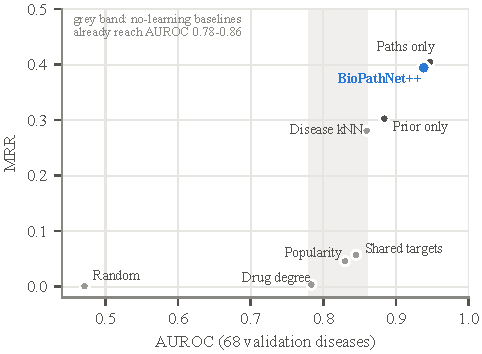
\includegraphics[width=\columnwidth]{fig_auroc_vs_mrr.pdf}
\caption{AUROC does not separate methods in this task: no-learning baselines reach 0.78--0.86, while ranking quality (MRR) differs by two orders of magnitude.}
\label{fig:auroc}
\end{figure}

\textbf{Ablations.} Paths alone reach a validation MRR of \PathsValidMrr{}, statistically tied with the full model (difference \DiffMainPathsValid{}, Wilcoxon $p$\,\PwilMainPathsValid). The prior channel alone reaches \PriorValidMrr{}. Hence path reasoning carries the predictive signal. The transfer channel does not raise the mean, but it reduces seed variance on the targets (sd \MainTargetsMrrSd{} vs.\ \PathsTargetsMrrSd{} for paths only). In single-seed ablations, the listwise softmax loss beats NBFNet's self-adversarial BCE (validation MRR \MainValidMrr{} vs.\ \BceValidMrr{}; Wilcoxon $p$\,\PwilMainBceValid). Restricting message passing to a BioPathNet-style background graph that drops tissue-expression and drug--drug edges removes \BrgEdgeCutPct\% of edges with unchanged accuracy (\BrgValidMrr{}; $p$\,\PwilMainBrgValid) and \BrgSpeedupPct\% shorter training steps.

\subsection{Does transfer come from autoimmune diseases?}
Removing all 123 autoimmune diseases from training leaves target MRR unchanged (\NoautoTargetsMrr{} without vs.\ \MainTargetsMrr{} with them; \NoautoSeeds{} seeds each; $p$\,\PwilMainNoautoTargets). On the 21 held-out autoimmune-area diseases the model reaches MRR \NoautoAreaMrr{} versus \NoautoKnnAreaMrr{} for disease $k$NN. The difference is consistent in direction (CI \DiffLoNoautoKnnArea{} to \DiffHiNoautoKnnArea) but not significant by the Wilcoxon test ($p$\,\PwilNoautoKnnArea). The hypothesis that the model transfers knowledge specifically from data-rich autoimmune diseases is therefore \emph{not} supported: the transferable signal comes from the pharmacology and biology of the whole KG.

\subsection{Case studies}
Table~\ref{tab:targets} lists per-target results. For PBC, ursodeoxycholic acid, the first-line therapy, ranks first in every seed. For MG, the four labelled cholinesterase inhibitors (ambenonium, neostigmine, pyridostigmine, distigmine) occupy ranks 1--4 in all seeds, and amifampridine, unlabelled in PrimeKG but tested in a completed phase~3 MG trial (NCT03304054), is fifth in two seeds. For SSc the labelled drugs aminobenzoic acid, benzoic acid and bosentan lead. For Sj\"ogren, labelled tear-substitute components and prednisolone are at the top, and lifitegrast, approved for dry-eye disease, enters the top 4 in two seeds. AIH fails by label rather than by model: PrimeKG lists a single off-label drug for AIH, while the model ranks prednisolone first in two of three seeds; corticosteroids of this class are the standard comparator in AIH trials (prednisone in NCT00838214). Corticosteroids rank highly for several diseases. This is clinically sensible, but it also reflects popularity bias.

\begin{table}[t]
\centering
\caption{Per-target MRR (seed mean). Best rank: highest-ranked labelled drug (seed 0). $^{*}$\,labelled in PrimeKG.}
\label{tab:targets}
\scriptsize
\setlength{\tabcolsep}{2.5pt}
\resizebox{\columnwidth}{!}{\begin{tabular}{lcccccl}
\toprule
Target & \#known & kNN & Paths only & BioPathNet++ & Best rank & Top-3 predictions (seed 0)\\
\midrule
PBC & 1 & 1.000 & 1.000 & 1.000 & 1 & Ursodeoxycholic acid$^{*}$, Doripenem, Cholic Acid\\
SSc & 5 & 0.041 & 0.437 & 0.452 & 1 & Benzoic acid$^{*}$, Bosentan$^{*}$, Limaprost\\
Sj\"ogren & 12 & 0.152 & 0.731 & 0.510 & 1 & Prednisolone$^{*}$, Polyethylene glycol 400$^{*}$, Propylene glycol$^{*}$\\
AIH & 1 & 0.001 & 0.002 & 0.002 & $>$100 & Prednisolone, Triamcinolone, Hydrocortisone\\
MG & 7 & 0.179 & 0.418 & 0.671 & 1 & Ambenonium$^{*}$, Neostigmine$^{*}$, Pyridostigmine$^{*}$\\
Crohn & 24 & 0.403 & 0.191 & 0.212 & 1 & Hydrocortisone$^{*}$, Triamcinolone$^{*}$, Cortisone acetate$^{*}$\\
\bottomrule
\end{tabular}}
\end{table}

\section{Discussion and Limitations}
The audit is the most transferable lesson: under random negatives and leaky graphs, near-perfect AUROC is reachable without learning. Our numbers are lower but measure a harder task. For context, BioPathNet reports indication MRR between about 0.2 and 0.8 across TxGNN's zero-shot disease areas~\cite{hu2026biopathnet}, a range that contains ours. These numbers are not directly comparable, however: their splits also remove 95\% of the held-out diseases' molecular edges, while ours remove families. We did not run TxGNN or BioPathNet on our split and make no head-to-head claim.

Limitations: (i) target labels are sparse (one drug each for PBC and AIH), so per-target metrics are noisy; (ii) the 68 validation diseases also select the epoch; the resulting optimism is \SelGapMainMin--\SelGapMainMax{} MRR for the full model, far below the gain over $k$NN, while the targets and area diseases are untouched by selection; (iii) new candidates are hypotheses that need clinical evidence; (iv) path explanations are not yet extracted.

\section{Conclusion}
Under a strict-family, full-ranking protocol, a path-based NBFNet model clearly outperforms strong similarity baselines for unseen diseases and recovers established therapies for several rare autoimmune diseases. Equally important, careful evaluation exposed leakage that inflated earlier results, and it showed that neither the transfer channel nor autoimmune-specific training data is the source of the gains. Code, splits and run logs are released for reproduction.

\section*{Acknowledgment}
% IEEE policy requires disclosure of AI-generated content; edit to describe actual use.
Generative AI tools were used to assist with code development, data analysis and language editing; all results were verified by the authors against the released run logs.

\bibliographystyle{IEEEtran}
\bibliography{references}

\end{document}
